\documentclass{article}
\usepackage{tikz}
\begin{document}
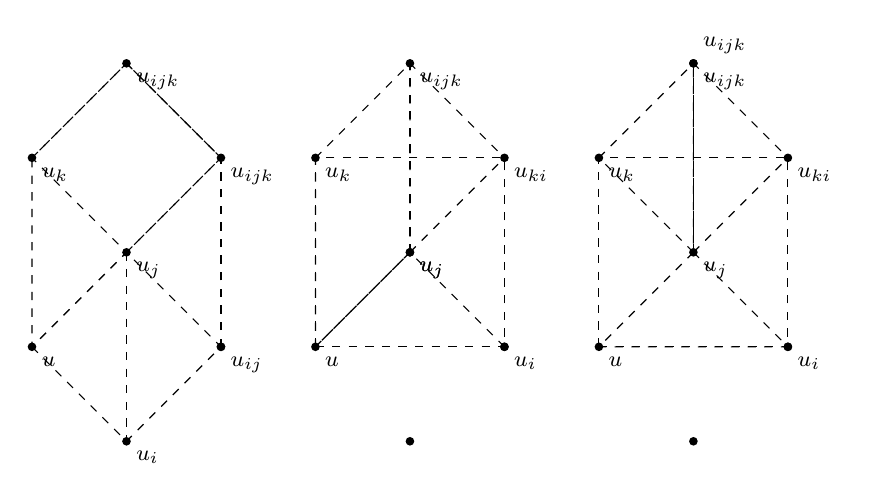
\begin{tikzpicture}[scale=1.2]
    \begin{scope}[xshift=0cm]
    \draw[dashed] (0,0)--(1,-1)--(2,0)--(1,1)--(0,0);
    \draw[dashed] (1,1)--(1,-1);
    \draw[dashed] (1,1)--(2,2)--(1,3)--(0,2)--(1,1);
    \draw[dashed] (1,3)--(2,2);
    \draw[dashed] (0,2)--(1,3)--(2,2)--(1,1)--(0,0)--(0,2);
    \draw[dashed] (2,0)--(2,2);
    \foreach \x/\y/\name in {0/0/u,1/-1/u_i,2/0/u_{ij},1/1/u_j,1/3/u_{ijk},0/2/u_k,2/2/u_{i j k},2/0/}
        \fill (\x,\y) circle (1.3pt) node[below right] {\footnotesize $\name$};
    \end{scope}

    \begin{scope}[xshift=3cm]
    \draw[dashed] (0,0)--(2,0)--(2,2)--(0,2)--(0,0);
    \draw[dashed] (0,2)--(1,3)--(2,2);
    \draw[dashed] (1,1)--(1,3);
    \draw[dashed] (1,1)--(2,2);
    \draw[dashed] (0,0)--(1,1)--(1,3);
    \draw[dashed] (1,1)--(0,0)--(0,2);
    \draw[dashed] (2,0)--(1,1);
    \foreach \x/\y/\name in {0/0/u,1/-1/,2/0/u_{i},1/1/u_j,1/3/u_{ijk},0/2/u_k,2/2/u_{k i},2/0/}
        \fill (\x,\y) circle (1.3pt) node[below right] {\footnotesize $\name$};
    \fill (1,1) circle (1.3pt) node[below right] {\footnotesize $u_j$}; % Redundant but for clarity
    \end{scope}

    \begin{scope}[xshift=6cm]
    \draw[dashed] (0,0)--(2,0)--(2,2)--(0,2)--(0,0);
    \draw[dashed] (0,2)--(1,3)--(2,2);
    \draw[dashed] (1,1)--(1,3);
    \draw[dashed] (1,1)--(2,2);
    \draw[dashed] (1,1)--(0,2);
    \draw[dashed] (1,1)--(0,0)--(2,0)--(1,1)--(1,3);
    \foreach \x/\y/\name in {0/0/u,1/-1/,2/0/u_{i},1/1/u_j,1/3/u_{ijk},0/2/u_k,2/2/u_{ki},2/0/}
        \fill (\x,\y) circle (1.3pt) node[below right] {\footnotesize $\name$};
    \fill (1,3) circle (1.3pt) node[above right] {\footnotesize $u_{ijk}$}; % Adjusting label position
    \end{scope}
\end{tikzpicture}
\end{document}